% ------------------------------------------------------------------------------
% TYPO3 CMS 8.0 - What's New - Chapter "Introduction" (German Version)
%
% @author	Michael Schams <schams.net>
% @license	Creative Commons BY-NC-SA 3.0
% @link		http://typo3.org/download/release-notes/whats-new/
% @language	German
% ------------------------------------------------------------------------------
% LTXE-CHAPTER-UID:		cb43d098-7bf9a537-bf3817c0-53a0f29f
% LTXE-CHAPTER-NAME:	Introduction
% ------------------------------------------------------------------------------

\section{Introduction}
\begin{frame}[fragile]
	\frametitle{Introduction}

	\begin{center}\huge{Introduction}\end{center}
	\begin{center}\huge{\color{typo3darkgrey}\textbf{Die Fakten}}\end{center}

\end{frame}

% ------------------------------------------------------------------------------
% LTXE-SLIDE-START
% LTXE-SLIDE-UID:		5db12b0d-3b71ed55-6242aa10-80df7cde
% LTXE-SLIDE-ORIGIN:	9e397afb-762f7061-0e0e0bd1-9836250e English
% LTXE-SLIDE-TITLE:		TYPO3 CMS 8.0 - The Facts
% ------------------------------------------------------------------------------
\begin{frame}[fragile]
	\frametitle{Einführung}
	\framesubtitle{TYPO3 CMS 8.0 - The Facts}

	\begin{itemize}
		\item Veröffentlichungsdatum: 22. März 2016
		\item Releasetyp: Sprint Release
		\item Vision: Start your engines
	\end{itemize}

	\begin{figure}
		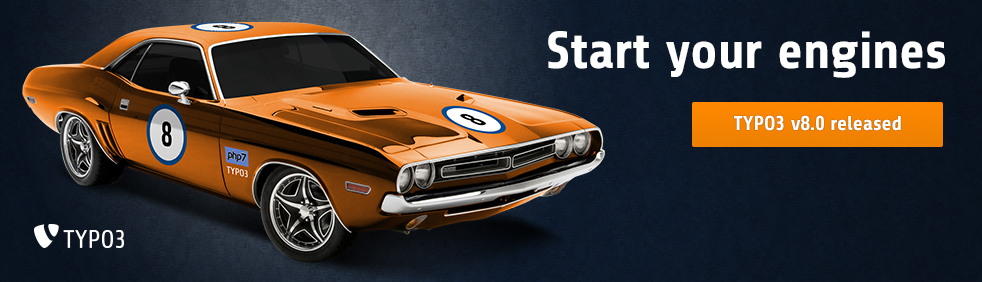
\includegraphics[width=0.95\linewidth]{Introduction/typo3cms80-banner.png}
	\end{figure}

\end{frame}

% ------------------------------------------------------------------------------
% LTXE-SLIDE-START
% LTXE-SLIDE-UID:		c63d7b42-d0c1166e-aea48a58-aa5834f3
% LTXE-SLIDE-ORIGIN:	737c8e9b-4ae60e26-6975ea72-21146dd0 English
% LTXE-SLIDE-TITLE:		System Requirements
% ------------------------------------------------------------------------------
\begin{frame}[fragile]
	\frametitle{Einführung}
	\framesubtitle{Systemvoraussetzungen}

	\begin{itemize}
		\item PHP:\tabto{3cm}v7.0.0
		\item MySQL:\tabto{3cm}v5.5.x - v5.7.x
		\item Festplattenplatz:\tabto{3cm}mindestens 200 MB
		\item PHP settings:

			\begin{itemize}
				\item \texttt{memory\_limit} >= 128M
				\item \texttt{max\_execution\_time} >= 240s
				\item \texttt{max\_input\_vars} >= 1500
				\item compilation option \texttt{-}\texttt{-disable-ipv6} must \underline{not} be used
			\end{itemize}

		\item Das Backend benötigt einen Microsoft Internet Explorer 11 oder später,
			Microsoft Edge, Google Chrome, Firefox, Safari oder jeden anderen modernen Browser

	\end{itemize}

\end{frame}

% ------------------------------------------------------------------------------
% LTXE-SLIDE-START
% LTXE-SLIDE-UID:		55c242b0-944111c4-210d0cc9-0a5676e5
% LTXE-SLIDE-ORIGIN:	90d2d3d1-f9d57661-dd01143b-10630416 English
% LTXE-SLIDE-TITLE:		Development And Release Timeline
% ------------------------------------------------------------------------------
\begin{frame}[fragile]
	\frametitle{Einführung}
	\framesubtitle{Release Zyklus}

	\begin{figure}
		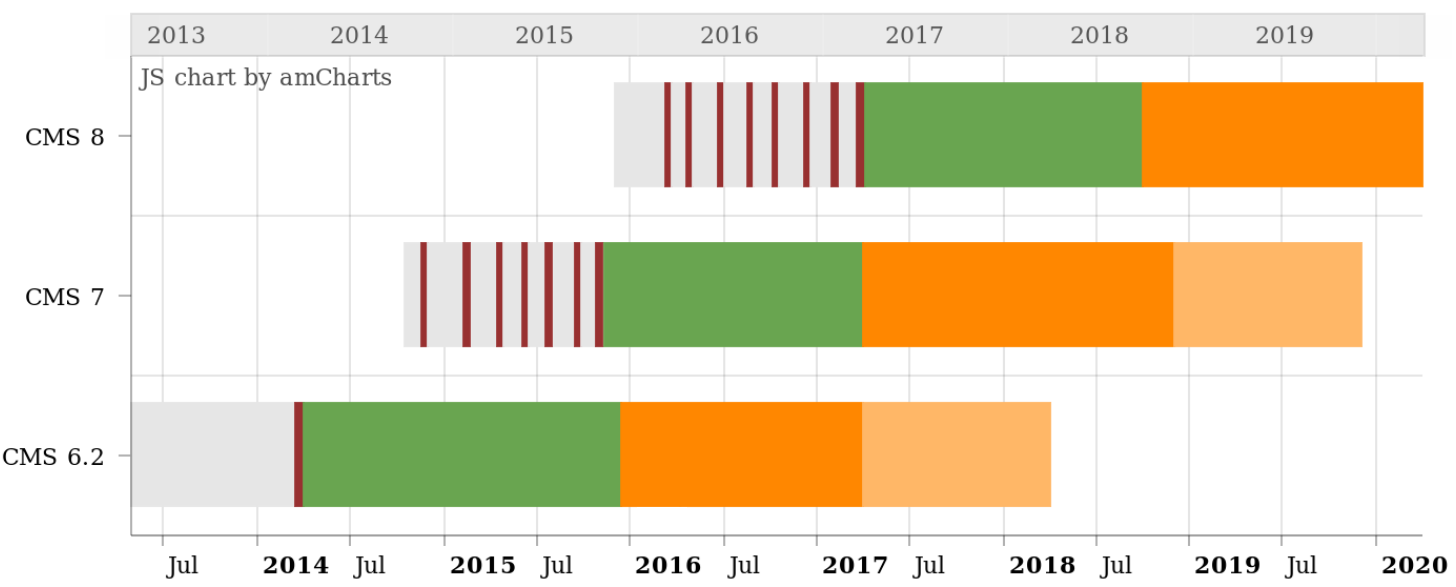
\includegraphics[width=0.90\linewidth]{Introduction/ReleaseAgenda.png}
	\end{figure}

\end{frame}

% ------------------------------------------------------------------------------
% LTXE-SLIDE-START
% LTXE-SLIDE-UID:		ab81e0c9-238689d7-a1da1d27-8bda97d9
% LTXE-SLIDE-ORIGIN:	13e0fd6a-fa50d02d-c15c4af0-f3996926 English
% LTXE-SLIDE-TITLE:		TYPO3 CMS Roadmap
% ------------------------------------------------------------------------------
\begin{frame}[fragile]
	\frametitle{Einführung}
	\framesubtitle{TYPO3 CMS Roadmap}

	Voraussichtliche Veröffentlichungen und deren Hauptfokus:

	\begin{itemize}

		\item
			\begingroup
				\color{typo3orange}
					v8.0 \tabto{1.1cm}22/Mar/2016\tabto{3.4cm}Adding last minute things
			\endgroup
		\item v8.1 \tabto{1.1cm}03/Mai/2016\tabto{3.4cm}Cloud Integration
		\item v8.2 \tabto{1.1cm}05/Jul/2016\tabto{3.4cm}Rich Text Editor
		\item v8.3 \tabto{1.1cm}30/Aug/2016\tabto{3.4cm}Frontend Editing on Steroids
		\item v8.4 \tabto{1.1cm}18/Okt/2016\tabto{3.4cm}\textit{to be determined}
		\item v8.5 \tabto{1.1cm}20/Dez/2016\tabto{3.4cm}Integrator Support
		\item v8.6 \tabto{1.1cm}14/Feb/2017\tabto{3.4cm}\textit{to be determined}
		\item v8.7 \tabto{1.1cm}04/Apr/2017\tabto{3.4cm}LTS Preparation

	\end{itemize}

	\smaller
		\url{https://typo3.org/typo3-cms/roadmap/}\newline
		\url{https://typo3.org/news/article/kicking-off-typo3-v8-development/}
	\normalsize

\end{frame}

% ------------------------------------------------------------------------------
% LTXE-SLIDE-START
% LTXE-SLIDE-UID:		b244c478-9ece1082-ecbe65bb-3f2d040e
% LTXE-SLIDE-ORIGIN:	06c6100a-69216610-618bde63-bbdc4eef English
% LTXE-SLIDE-TITLE:		Installation
% ------------------------------------------------------------------------------
\begin{frame}[fragile]
	\frametitle{Einführung}
	\framesubtitle{Installation}

	\begin{itemize}
		\item Empfohlene Installationsschritte unter Linux/Mac OS X\newline
			(DocumentRoot ist beispielsweise \texttt{/var/www/site/htdocs}):
		\begin{lstlisting}
			$ cd /var/www/site
			$ wget --content-disposition get.typo3.org/8.0
			$ tar xzf typo3_src-8.0.0.tar.gz
			$ cd htdocs
			$ ln -s ../typo3_src-8.0.0 typo3_src
			$ ln -s typo3_src/index.php
			$ ln -s typo3_src/typo3
			$ touch FIRST_INSTALL
		\end{lstlisting}

		\item Symbolische Links unter Microsoft Windows:

			\begin{itemize}
				\item unter Windows XP/2000 kann \texttt{junction} benutzt werden
				\item unter Windows Vista und Windows 7 kann \texttt{mklink} benutzt werden
			\end{itemize}

	\end{itemize}
\end{frame}

% ------------------------------------------------------------------------------
% LTXE-SLIDE-START
% LTXE-SLIDE-UID:		91a19941-5d54733a-7c43fa76-9b399ed0
% LTXE-SLIDE-ORIGIN:	b878899c-e4b09ddf-4c0ea575-9e0900ad English
% LTXE-SLIDE-TITLE:		Upgrade to TYPO3 CMS 7
% ------------------------------------------------------------------------------
\begin{frame}[fragile]
	\frametitle{Einführung}
	\framesubtitle{Upgrade zu TYPO3 CMS 8.x}

	\begin{itemize}
		\item Upgrades sind nur von TYPO3 CMS 7.6 LTS möglich
		\item TYPO3 CMS < 7.6 LTS sollte man zuerst auf TYPO3 CMS 7.6 LTS aktualisieren
	\end{itemize}

	\begin{itemize}

		\item Upgrade-Anleitung:\newline
			\smaller\url{http://wiki.typo3.org/Upgrade#Upgrading_to_8.0}\normalsize
		\item Official TYPO3 guide "TYPO3 Installation and Upgrading":
			\smaller\url{http://docs.typo3.org/typo3cms/InstallationGuide}\normalsize
		\item Generelles Vorgehen:
			\begin{itemize}
				\item Prüfen, ob Mindestvoraussetzungen erfüllt sind \small(PHP, MySQL, etc.)
				\item Das \textbf{deprecation\_*.log} der TYPO3 Instanz durchsehen
				\item Sämtliche Extensions auf den aktuellsten Stand bringen
				\item Neuen TYPO3 Quellcode entpacken und im Install Tool den Upgrade Wizard ausführen
				\item Startup Modul von Backend Benutzern überprüfen (optional)
			\end{itemize}
	\end{itemize}

\end{frame}

% ------------------------------------------------------------------------------

% ------------------------------------------------------------------------------
% LTXE-SLIDE-START
% LTXE-SLIDE-UID:		0f79bfdb-bc225866-01cdfa1e-c372c4af
% LTXE-SLIDE-ORIGIN:	e4b09ddf-4c0ea575-9e0900ad-b878899c English
% LTXE-SLIDE-TITLE:		PHP Version 7
% ------------------------------------------------------------------------------
\begin{frame}[fragile]
	\frametitle{Einführung}
	\framesubtitle{PHP Version 7}

	\begin{itemize}

		\item PHP 7.0 ist die minimal mögliche Version für TYPO3 CMS 8.x
		\item TYPO3 wird kontinuierlich weitere PHP 7 Releases unterstützen, sobald diese veröffentlicht werden
		\item Diese Version beschleunigt das gesamte System signifikant

		\item Nicht nur Backend-Redakteure werden das deutlich beschleunigte Interface bemerken, auch der Aufruf des Caches im Frontend ist nun unter 7ms möglich, was ein Geschwindigkeitswachstum von 40\% gegenüber PHP 5.5 bedeutet

		\item Zeitgleicht wurden neue PHP 7 Features in den Core integriert, wie beispielsweise die Verwendung der kryptografischen Pseudo-Zufalls-Generatoren

	\end{itemize}

\end{frame}

% ------------------------------------------------------------------------------
